\documentclass{article}
\usepackage[utf8]{inputenc}
\usepackage{natbib}
\usepackage{amsmath}
\usepackage{amssymb}
\usepackage{graphicx}

\title{\textbf{MATH 307: Individual Homework 9}}
\author{John Mays}
\date{03/08/21, Dr. Guo}

\begin{document}

\maketitle

\section*{Problem 1}
Default inner product in $\mathbb{C}^3$:
\begin{equation*}
    \forall u,v \in \mathbb{C}^3, \langle u,v \rangle = |u_1||v_1|+|u_2||v_2|+|u_3||v_3|
\end{equation*}
The induced norm is defined as:
\begin{equation*}
    \begin{split}
        ||u||&=\sqrt{\langle u, u \rangle}\\
        &=\sqrt{|u_1||u_1|+|u_2||u_2|+|u_3||u_3|}\\
        &={\sqrt{|u_1|^2+|u_2|^2+|u_3|^2}}
    \end{split}
\end{equation*}
The 2-norm is defined as:
\begin{equation*}
    \begin{split}
        ||u||_2&= \left( \sum_{i=1}^{3}|u_i|^{2}\right)^{\frac{1}{2}}\\
        &=\sqrt{\sum_{i=1}^{3}|u_i|^{2}}\\
        &={\sqrt{|u_1|^2+|u_2|^2+|u_3|^2}}
    \end{split}
\end{equation*}
Therefore the induced norm is equal to the 2-norm:
\begin{equation*}
    \forall u \in \mathbb{C}^3, ||u||_{ind}=||u||_{2}
\end{equation*}
$||u||=\sqrt{|1+i|^2+|2i|^2+|3+i|^2}=\sqrt{\sqrt{2}^2+2^2+\sqrt{10}^2}\\
=\sqrt{2+4+10}=\sqrt{16}=4$\\
$d(u,v)=||u-v||=||(i,-3+3i,3+2i)||=\sqrt{|i|^2+|-3+3i|^2+|3+2i|^2}=\sqrt{1+18+13}=\sqrt{32}=4\sqrt{2}$
\pagebreak
\section*{Problem 2}
\subsubsection*{1-norm:}
$||x||_1=|x_1|+|x_2|=1$
\begin{figure}[htp]
    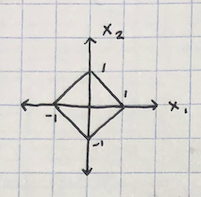
\includegraphics[width=3cm]{1norm.png}
\end{figure}
\subsubsection*{2-norm:}
$||x||_2=\sqrt{|x_1|^2+|x_2|^2}=1$\\ 
$||x||_2=|x_1|^2+|x_2|^2=1$
\begin{figure}[htp]
    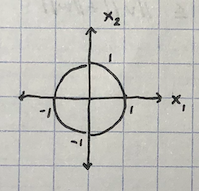
\includegraphics[width=3cm]{2norm.png}
\end{figure}
\subsubsection*{$\infty$-norm:}
$||x||_\infty=\max{(x_1,x_2)}=1$
\begin{figure}[htp]
    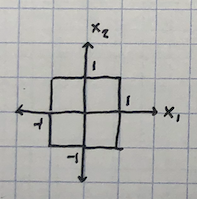
\includegraphics[width=3cm]{infnorm.png}
\end{figure}
\pagebreak
\subsubsection*{1 on all norms:}
Composing the three norms on top of each other,

\begin{figure}[htp]
    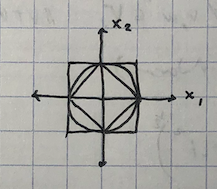
\includegraphics[width=3cm]{composed.png}
\end{figure}
we can see that four points on the $x_1$, $x_2$ plane qualify as 1 for all norms: $(0,1),(1,0),(0,-1),(-1,0)$.



\end{document}